% Figure 16: design procedure; screening decisions precede coupled verification.
\begin{tikzpicture}[font=\pesfigfont,>=latex,line width=.5pt,
 designstep/.style={draw,fill=white,align=center,text width=2.75cm,
 minimum height=6mm,inner sep=1.5mm},
 result/.style={designstep,fill=gray!12},
 panel/.style={draw,rounded corners=2pt},
 small/.style={font=\pesfigfont,align=center}]
\node[draw,fill=gray!5,align=center,text width=16.5cm,minimum height=12mm] (spec) at (8.4,15.8)
 {\textbf{Traction-drive specification and system constraints}\\
 $P=300$ kW, $V_{\rm dc}=1200$ V, $M\leq1.15$, $\eta_{\rm stage}\geq99.5\%$, $\Delta v_{\rm pp}\leq4\%$;
 mission, voltage margin, temperature and package limits};
\foreach \x/\col in {0/pesblue,3.4/green!50!black,6.8/pesred,10.2/violet,13.6/teal!70!black}{
 \draw[panel,\col,fill=\col!3] (\x,8.0) rectangle ++(3.2,6.8);
 \draw[->] (\x+1.6,15.2)--(\x+1.6,14.8);
}
\node[small,text=pesblue] at (1.6,14.5) {\textbf{Voltage class and device}};
\node[designstep] (a1) at (1.6,13.6) {$R_{\rm DS(on)}(T)$, $Q_{\rm oss}$\\package and voltage rating};
\node[designstep] (a2) at (1.6,12.0) {$\tau_d=R_{\rm DS(on)}Q_{\rm oss}/V_{\rm test}$\\integer $N$; transient margin};
\node[result] (a3) at (1.6,10.4) {EPC2361, 100 V\\$N=16$, $V_c=75$ V};
\node[small,text width=2.8cm] at (1.6,8.65) {Low resistance and output charge; check system overhead};
\draw[->] (a1)--(a2);\draw[->] (a2)--(a3);
\node[small,text=green!50!black] at (5,14.5) {\textbf{Layout and gate drive}};
\node[designstep] (b1) at (5,13.6) {Sharing sensitivity\\$L_G$, $L_{CS}$, timing, $V_{\rm th}$};
\node[designstep] (b2) at (5,12.0) {Mirrored commutation loops\\star-connected gates; Kelvin};
\node[result] (b3) at (5,10.4) {One half-bridge driver\\per two parallel devices/switch};
\node[small,text width=2.8cm] at (5,8.65) {Match paths within pairs and timing between drivers};
\draw[->] (b1)--(b2);\draw[->] (b2)--(b3);
\node[small,text=pesred] at (8.4,14.5) {\textbf{Parallel-device count}};
\node[designstep] (c1) at (8.4,13.6) {$P_{\rm cond}\propto1/n_p$\\$P_{\rm sw}(n_p)$, copper, auxiliaries};
\node[designstep] (c2) at (8.4,12.0) {Loss and thermal budget\\versus device/driver count};
\node[result] (c3) at (8.4,10.4) {$n_p=4$ candidate\\two drivers per phase leg};
\node[small,text width=2.8cm] at (8.4,8.65) {Two repeated two-parallel blocks; verify inter-block sharing};
\draw[->] (c1)--(c2);\draw[->] (c2)--(c3);
\node[small,text=violet] at (11.8,14.5) {\textbf{DC link and frequency}};
\node[designstep] (d1) at (11.8,13.6) {Three-phase $i_C$, voltage ripple\\rms loading; dc-bias derating};
\node[designstep] (d2) at (11.8,12.0) {$C$, ESR/ESL and $R(f),L(f)$\\losses versus current ripple};
\node[result] (d3) at (11.8,10.4) {50-kHz evaluation point\\464.4 $\mu$F effective/cell};
\node[small,text width=2.8cm] at (11.8,8.65) {4.12\% worst evaluated ripple: increase bank for 4\% limit};
\draw[->] (d1)--(d2);\draw[->] (d2)--(d3);
\node[small,text=teal!70!black] at (15.2,14.5) {\textbf{Machine and integration}};
\node[designstep] (m1) at (15.2,13.6) {Winding groups, $L$, harmonics\\insulation and common mode};
\node[designstep] (m2) at (15.2,12.0) {Shared cooling, thermal coupling\\busbars, phase leads, volume};
\node[result] (m3) at (15.2,10.4) {16 three-phase cells\\48 legs; axial end connections};
\node[small,text width=2.8cm] at (15.2,8.65) {Machine model constrains $f_{\rm sw}$; packaging constrains cooling};
\draw[->] (m1)--(m2);\draw[->] (m2)--(m3);
\foreach \a/\b in {a3/b3,b3/c3,c3/d3}\draw[->] (\a.east)--(\b.west);
\draw[<->] (d3.east)--(m3.west);
\draw[panel,fill=orange!3] (0,4.75) rectangle (16.8,7.45);
\node[small,anchor=west] at (.2,7.17) {\textbf{Coupled verification using consistent geometry and operating conditions}};
\foreach \x/\head/\img/\desc in {
 1.4/PCB placement/kicad_3d.png/{Two-parallel block},
 4.2/Q3D extraction/q3d_model.png/{$R(f)$, $L(f)$; loops},
 7.0/Circuit simulation/switching_thumb.png/{Energy, stress, sharing},
 9.8/Loss model/losses_thumb.png/{Device and network losses},
 12.6/Thermal model/icepak_model.png/{Device, PCB, cooling}}{
 \node[small] at (\x,6.78) {\textbf{\head}};
 \node at (\x,5.95) {\includegraphics[width=2.25cm,height=13mm,keepaspectratio]{Figures/Section-CaseStudy/\img}};
 \node[small,text width=2.4cm] at (\x,5.12) {\desc};
}
\node[small] at (15.4,6.78) {\textbf{Cell integration}};
\node at (15.4,5.95) {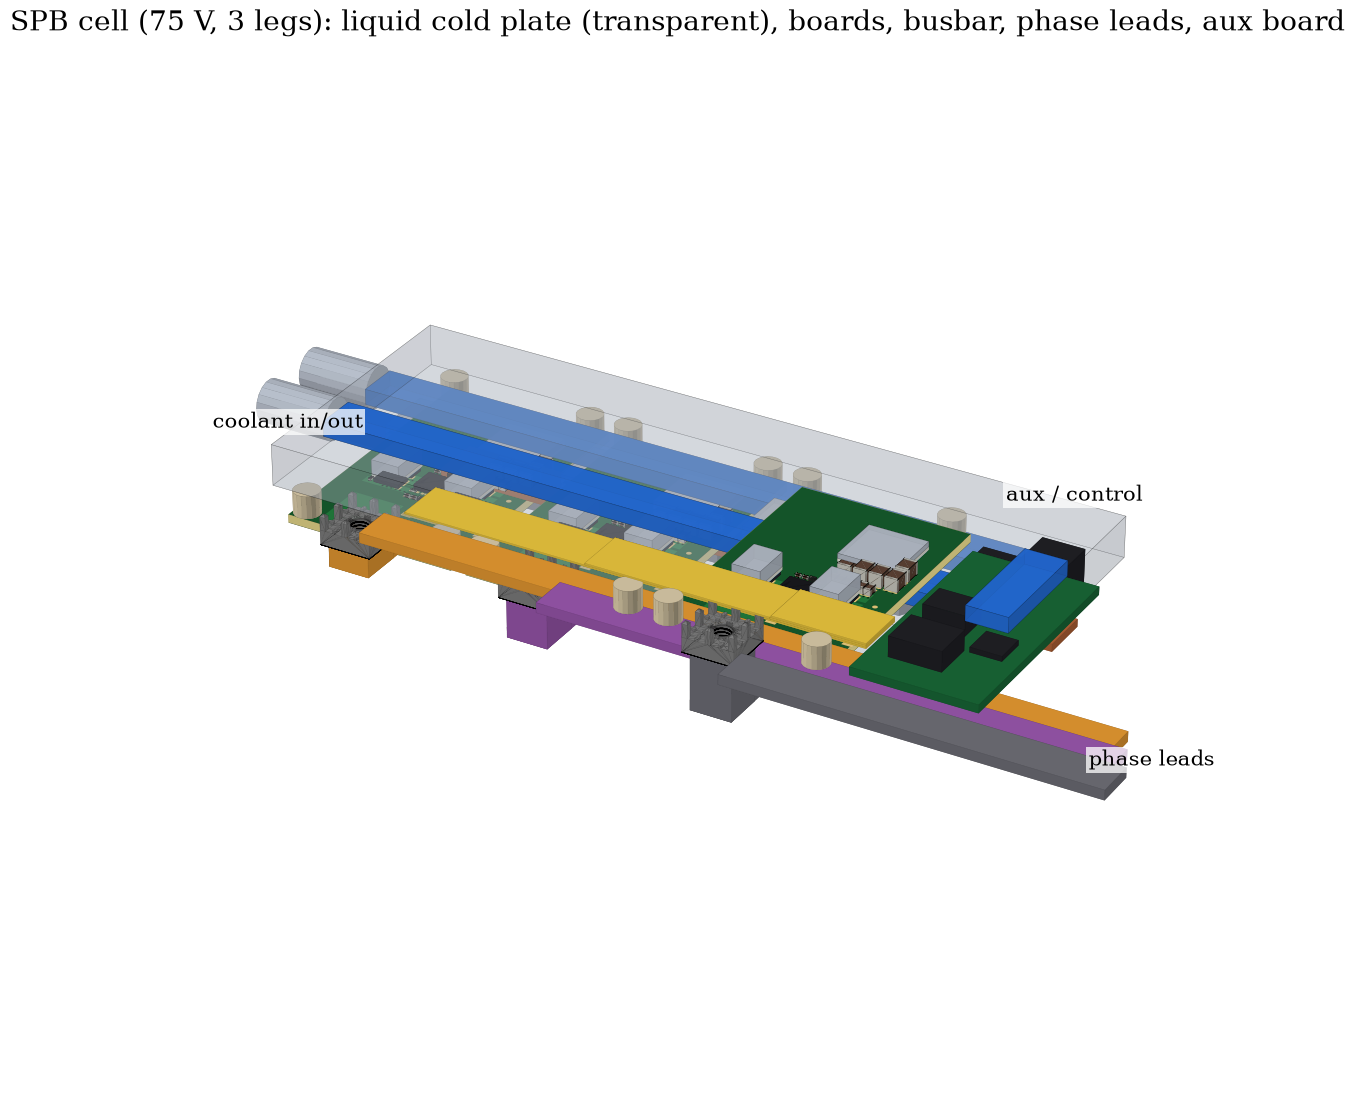
\includegraphics[width=2.25cm,height=13mm,keepaspectratio,
 trim=68bp 100bp 38bp 108bp,clip]{Figures/Section-CaseStudy/cell_iso.png}};
\node[small,text width=2.4cm] at (15.4,5.12) {Shared cooling\\busbars and leads};
\foreach \x in {1.6,5.0,8.4,11.8,15.2}\draw[->] (\x,8.0)--(\x,7.45);
\foreach \x in {1.4,4.2,7.0,9.8,12.6}\draw[->] (\x+1.16,5.95)--(\x+1.64,5.95);
\node[draw,align=center,fill=gray!6,text width=16.4cm,minimum height=9mm] (check) at (8.4,3.9)
 {\textbf{All constraints met?} Voltage/gate margins, efficiency, ripple, temperature, sharing and output quality\\
 Yes: prototype and motor validation (pending). No: revise $N$, $n_p$, layout, gate drive, $C_{\rm dc}$, $f_{\rm sw}$ or cooling.};
\draw[->] (8.4,4.75)--(check.north);
\draw[->,pesred,dashed] (check.east)--(17.05,3.9)--(17.05,15.12)--(5,15.12)--(5,14.8);
\end{tikzpicture}
